\documentclass[a4paper, 12pt]{article}
\usepackage{amsthm}
\usepackage{amsmath}
\DeclareMathOperator*{\argmax}{argmax}
\DeclareMathOperator*{\argmin}{argmin}

\usepackage[utf8]{inputenc}
\usepackage[T1]{fontenc}
\usepackage[english]{babel}
\usepackage{amsmath, amssymb}
\usepackage{graphicx}
\usepackage{listings}
\usepackage[margin=0.75in, top=0.75in, bottom=0.75in]{geometry}  % Reduce all margins
\usepackage{color}
\usepackage{float}
\usepackage{hyperref}
\newtheorem{theorem}{Theorem}


% Define colors
\definecolor{myblue}{RGB}{0, 0, 128}
\setlength{\parindent}{0pt}



% Define code listing settings
\lstset{
    basicstyle=\ttfamily\small,
    breaklines=true,
    numbers=left,
    numberstyle=\tiny,
    frame=single,
    language=Python,
}

\title{Expert Advice Problem as MDP}
\author{Hadar Tal}
\date{\today}

\begin{document}

\maketitle

\section*{Introduction}

In this document, we will describe the expert problem as a Markov Decision Process (MDP). 
We will give definitions for MDP, the expert problem, and the MDP for the expert problem.


\section*{Markov Decision Process}

A Markov Decision Process (MDP) is a tuple $(S, A, P_{s,a}(\cdot) , R_s(\cdot), \gamma)$, where:
\begin{itemize}
    \item $S$ is the state space.
    \item $A$ is the action space.
    \item $P_{s,a}(\cdot)$ is the transition probability function, $P_{s,a}(s') = \mathbb{P}(s_{t+1} = s' | s_t = s, a_t = a)$.
    \item $R_s(\cdot)$ is the reward function, $R_s(a) = \mathbb{E}[r_{t+1} | s_t = s, a_t = a]$.
    \item $\gamma$ is the discount factor.
\end{itemize}



\section*{Prediction from Expert Advice Problem}

In the Prediction from Expert Advice problem, also known as the prediction with expert advice problem, 
a learner seeks to make predictions or decisions based on the advice provided by a set of experts. 
Formally, the problem is defined as follows (for the binary prediction case):

\begin{itemize}
    \item \textbf{Time}: The problem unfolds over discrete time steps $t = 1, 2, ..., T$.

    \item \textbf{Events}: At each time $t$, one of two events occurs, denoted as $A$ or $B$.

    \item \textbf{Experts}: Let $\mathcal{E} = \{1, 2, ..., N\}$ denote the set of experts. 
    Each expert $i \in \mathcal{E}$ provides a prediction $p_t^i \in \{A, B\}$ for the event at time $t$.
    
    \item \textbf{Learner}: The learner receives the predictions from the experts and must make its own prediction $\hat{p}_t \in \{A, B\}$ 
    for the event at time $t$.  The learner's goal is to maximize its cumulative reward over time by making accurate predictions.
    
    \item \textbf{Outcome}: At each time $t$, the outcome of the event $q_t$ is revealed as either $A$ or $B$. 
    The learner's performance is evaluated based on its prediction and the actual outcome - if the learner's prediction is correct, 
    the reward is $1$, otherwise the reward is $0$.
    We consider the case where the outcomes are chosen by an adversary, i.e., the outcomes are not stochastic and are chosen to minimize 
    the learner's reward.
    In this case, the adversary has unlimited advantage over the learner, and we consider the learner's performance in terms of regret.

    \item \textbf{Regret}: The regret of the learner at time $T$ with respect to an expert $i$ is defined as:
    \[
    Regret_T(i) = \sum_{t=1}^T \mathbb{I}(p_t^i = q_t) - \mathbb{I}(\hat{p}_t = q_t) 
    \]
    where $\mathbb{I}(\cdot)$ is the indicator function. The regret measures the difference between the learner's performance 
    and the performance of expert $i$.
    We define the learner's regret as the maximum regret over all experts:
    \[
    Regret_T = \max_{i \in \mathcal{E}} Regret_T(i)
    \]

\end{itemize}


\section*{Online Markov Decision Processes (Even-Dar et al. 2006)}

Previous work by Eyal Even-Dar et al. considered adversarial rewards in the context of Markov Decision Processes (MDPs).
They consider an MDP with state space $S$, initial state distribution $d_1$ over $S$, action space $A$, 
state transition probabilities $\{P_{s,a}(\cdot)\}$, and a sequence of reward functions $r_1, r_2, \ldots, r_T$, 
where $r_t$ is the (bounded) reward function at time step $t$ mapping $S \times A$ into $[0, 1]$.

The goal is to maximize the sum of undiscounted rewards over a $T$-step horizon. 
They assume the agent has complete knowledge of the transition model $P$, but at time $t$, 
the agent only knows the past reward functions $r_1, r_2, \ldots, r_{t-1}$. 
Hence, an algorithm $A$ is a mapping from $S$ and the previous reward functions $r_1, \ldots, r_{t-1}$ to a probability distribution over actions, 
where $A(a|s, r_1, \ldots, r_{t-1})$ is the probability of taking action $a$ at time $t$.

They define the return of an algorithm $A$ as:
\[
V_{r_1, r_2, \ldots, r_T}(A) = \frac{1}{T} \mathbb{E} \left[ \sum_{t=1}^{T} r_t(s_t, a_t) \right],
\]
where $a_t \sim A(a|s_t, r_1, \ldots, r_{t-1})$ and $s_t$ is the random variable representing the state at time $t$, 
starting from initial state $s_1 \sim d_1$ and following actions $a_1, a_2, \ldots, a_{t-1}$.

They aim to find an algorithm $A$ that achieves a large reward $V_{r_1, \ldots, r_T}(A)$ regardless of how the adversary 
chooses the reward functions. 
In general, this is not possible, and, as in the standard experts setting, they desire that their algorithm competes favorably 
against the best fixed stationary policy $\pi(a|s)$ in hindsight.

They define the regret of an algorithm $A$ as:
\[
Regret_T(A) = \max_{\pi} \left\{ \frac{1}{T} \mathbb{E} \left[ \sum_{t=1}^{T} r_t(s_t, \pi(s_t)) \right] - \frac{1}{T} \mathbb{E} \left[ \sum_{t=1}^{T} r_t(s_t, a_t) \right] \right\}
\]
where the maximum is taken over all fixed stationary policies $\pi(a|s)$.

\medskip
Great algorithms for this setting are the Follow-the-Perturbed-Leader (FPL) algorithm and MDP-E (MDP with Expert Advice) algorithm.
The field of online MDPs was further developed and explored in the literature, however, in our case where we have 2 experts and binary predictions,
we can define the problem as a simple MDP and solve it using standard MDP algorithms, by exploiting the structure of the 
problem and the limitations of the adversary.

\section*{MDP for 2 Experts}


We define for each time step $t$ the state space 
$S_t = \{ [ \mathbb{R}_1 ,  \mathbb{R}_2 ] : \mathbb{R}_1, \mathbb{R}_2 \in \mathbb{N}^+ , \mathbb{R}_1 + \mathbb{R}_2 = t \}$,  
where $\mathbb{R}_1$ and $\mathbb{R}_2$ are the number of steps that were made during time steps $1, 2, \ldots, t$ by experts $1$ and $2$, respectively.

For each time step $t$, the feasible actions are $A_t = \{p_t^1, p_t^2\}$, where $p_t^i$ is the prediction of expert $i$ at time $t$.

\medskip

\begin{theorem}

The transition probabilities $P_{s,a}(\cdot)$ are deterministic, and depend on the action $a$ and the current state $s$.
For each state $s_t = [ \mathbb{R}_1 ,  \mathbb{R}_2 ]$, and action If $a_t = p_t^1$, then $s_{t+1} = [ \mathbb{R}_1 + 1 ,  \mathbb{R}_2 ]$ 
otherwise $[ \mathbb{R}_1 ,  \mathbb{R}_2 + 1 ]$.

\end{theorem}

\medskip 

Although the transition probabilities are deterministic, since the outcomes of the events are chosen by an adversary, 
we would might think that the reward function $R_s(\cdot)$ for the regret of the learner is non-deterministic.
However, we can define the reward function as deterministic, due to the fact that in each state it must select an outcome 
that will maximize the learner's regret.

\begin{theorem}

    let $s_t = [ \mathbb{R}_1 ,  \mathbb{R}_2 ]$ be the state at time $t$, and $s_{t+1} = [ \mathbb{R}_1' ,  \mathbb{R}_2' ]$ be the state at time $t+1$
    after taking action $a_t = p_t^i$.
    The reward function $R_s(\cdot)$ is defined as:
    \[
    R_s(a_t) = \begin{cases} 
        -1 & \text{if } \max\{ \mathbb{R}_1' ,  \mathbb{R}_2' \} = \max\{ \mathbb{R}_1 ,  \mathbb{R}_2 \} \\
        0 & \text{if } otherwise
    \end{cases}
    \]

\end{theorem}

\begin{proof}
    We will split the proof into two cases:
    \begin{itemize}
        \item If $\max\{ \mathbb{R}_1' ,  \mathbb{R}_2' \} = \max\{ \mathbb{R}_1 ,  \mathbb{R}_2 \}$, \ 
        W.L.O.G, let's assume that $\mathbb{R}_1 \gneq \mathbb{R}_2$.
        We can assume that, since equality will contradict that the maximum is the same.
        In this case, $a_t = p_t^2$. Since $Regret_T$ is the performance with respect to the two experts, 
        the optimal adversary will select the outcomes $q^1, \dots, q^T$ as

        \[ \argmax_{q^1, \dots , q^T} \max_{i \in \{1,2\}}  \left\{ \sum_{t=1}^T \mathbb{I}(p_t^i = q_t) - \mathbb{I}(\hat{p}_t = q_t) \right\} \]
        
        In this case, for any adversarial selection of an outcome $q_t$ the regret stay be the same, 
        since the overall regret will be based on the number of times the learner didn't follow expert 2 
        (it can achieve larger regert value since we followed it less during the time steps).

        

        \item If $\max\{ \mathbb{R}_1' ,  \mathbb{R}_2' \} \neq \max\{ \mathbb{R}_1 ,  \mathbb{R}_2 \}$ - 
        lets assume W.L.O.G that $\mathbb{R}_1' > \mathbb{R}_2'$.
        Then the adversary will select the outcome at time $t$ as $q_t = p_t^2$.
    \end{itemize}

\end{proof}


\bigskip

MDP $M_e$ for the 2 Experts Problem is the tuple $(S, A, P_{s,a}(\cdot) , R_s(\cdot), \gamma)$, where:
\begin{itemize}
    \item $S = \{ [ \mathbb{R}_1 ,  \mathbb{R}_2 ] : \mathbb{R}_1, \mathbb{R}_2 \in \mathbb{N}^+ \}$ 
    \item $A =  \cup_{t=1}^T \{p_t^1, p_t^2\}$ 
    \item $P_{s,a}(\cdot)$ is the transition probability function, as defined in Theorem 1.
    \item $R_s(\cdot)$ is the reward function, as defined in Theorem 2.
    \item $\gamma$ = 1 (undiscounted).
\end{itemize}

A figure of the MDP for the 2 Experts Problem for $T=3$ is shown in Figure \ref{fig:MDP}.
\begin{figure}[H]
    \centering
    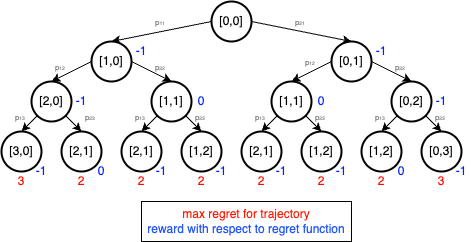
\includegraphics[width=0.5\textwidth]{MDP.png}
    \caption{MDP for the 2 Experts Problem for $T=3$}
    \label{fig:MDP}
\end{figure}

Simple algorithms for solving the MDP $M_e$ are Value Iteration using the Bellman Equation, 
or Dynamic Programming using the fact that the we want to minimize the regret. 



\end{document}

